\chapter{Output modules}
\label{chap:Output}

\section{DAC output}

\begin{figure}[h!]
    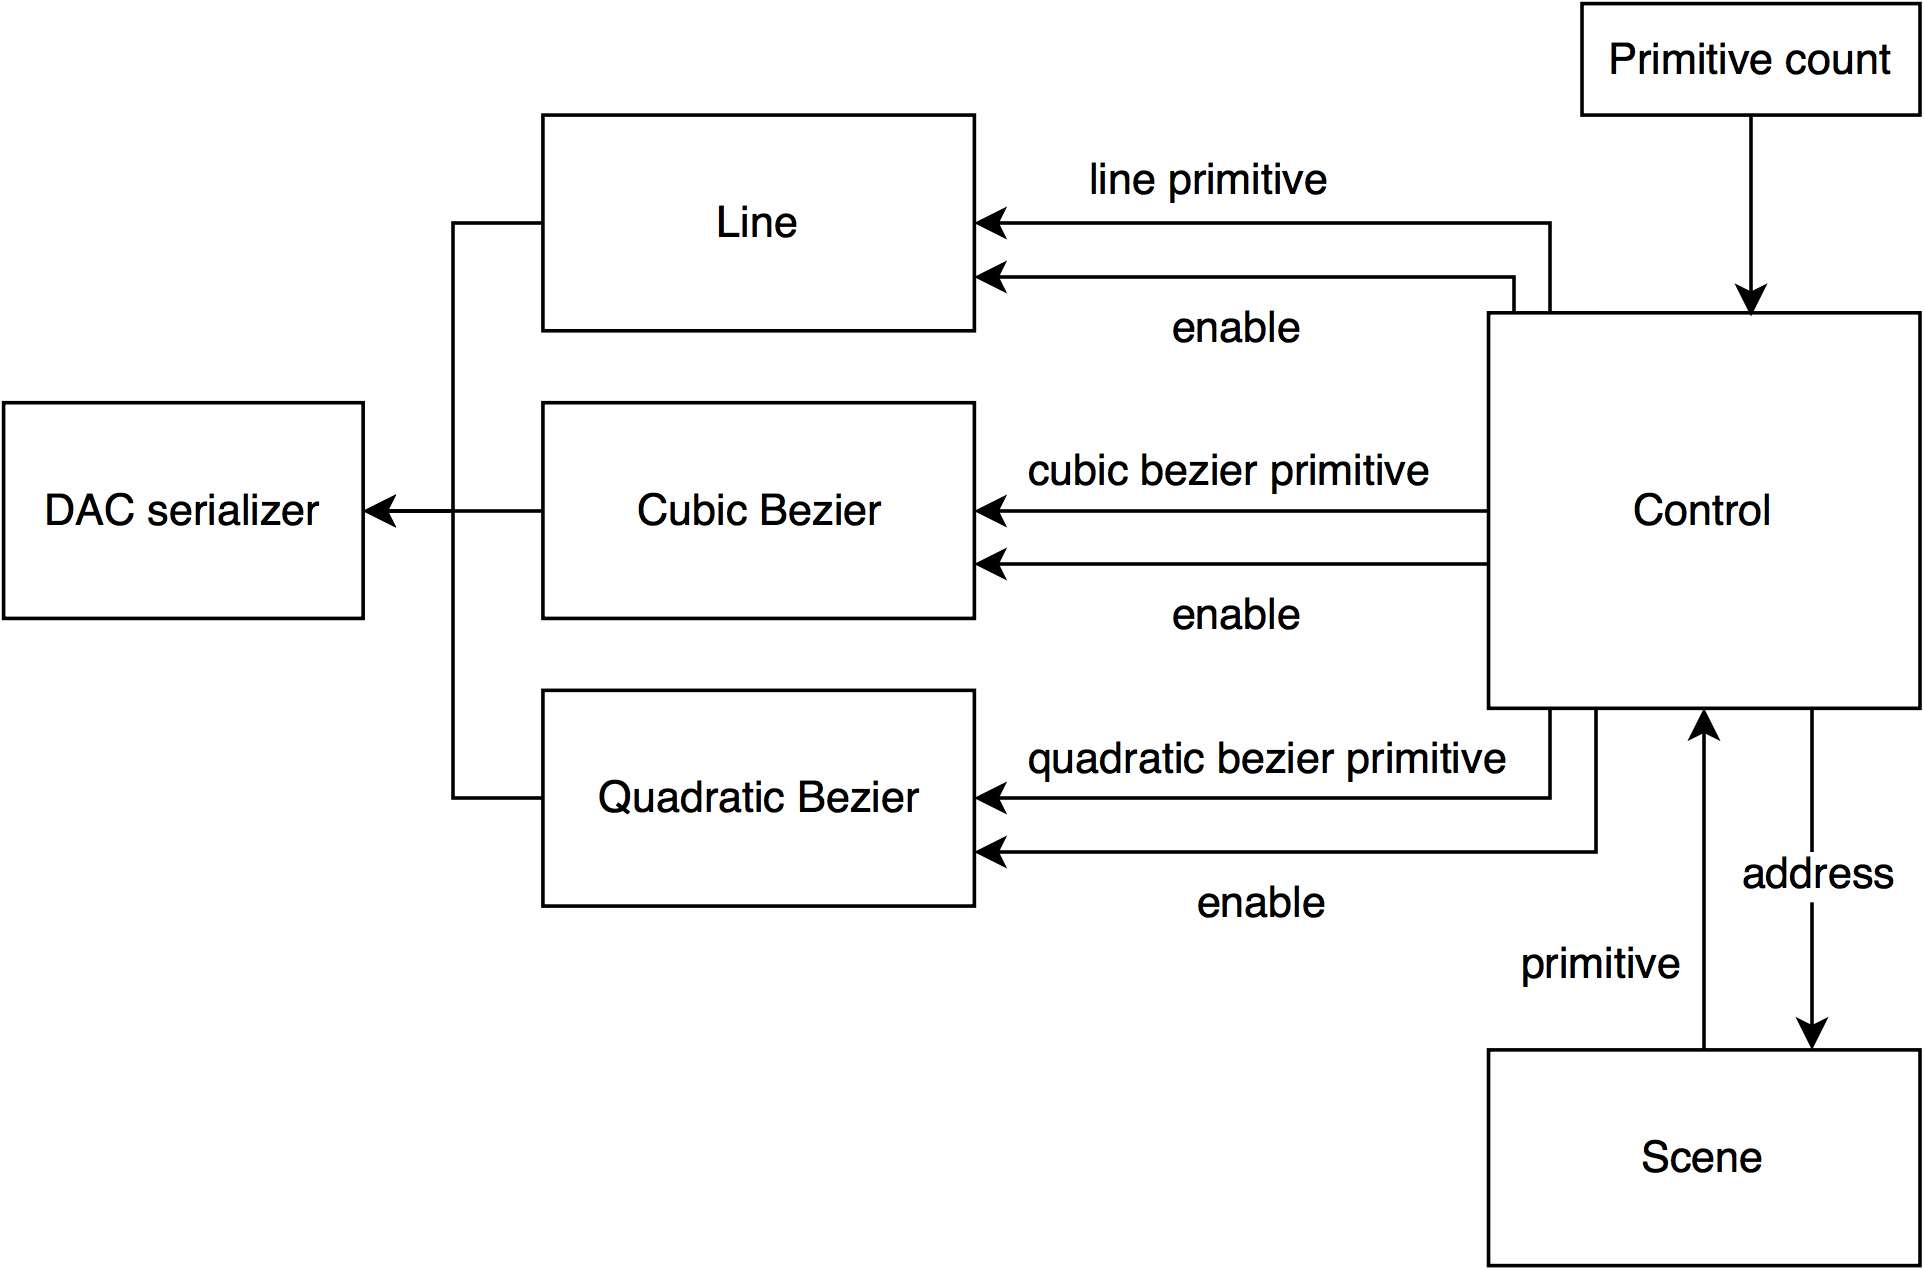
\includegraphics[width=\linewidth]{images/dac-output.png}
    \caption{RTL sketch of the \vthreek DAC output module.}
    \label{fig:dac-output}
\end{figure}

The primary output of the processor is the analogue one.
This output is driven by two DACs that get their data from a core on the FPGA.
The DACs need a clock, data, and sync signal to operate. 
Clock and sync signals are shared between the DACs so they operate synchronously. 

The parallel to serial converter takes a 32-bit signal as input.
This signal represents the x,y-coordinate pair of a point that is to be drawn on the oscilloscope.
The converter splits the signal into its x and y components and clocks them out synchronously to their respective DACs.

\section{Raster output}

This output uses HDMI to output a rasterized image of the internal vector representation.
In order to drive this output each primitive in the scene memory needs to be rasterized into a frame-buffer that is in turn TMDS encoded before it is sent over HDMI to a display.